\documentclass[../main.tex]{subfiles}

\begin{document}
Before delving into the design and optimization of our measuring circuit,
we need some theoretical context. First we will do a light overview of the
operating principles of an SET and how to use it to measure spin, then we will
pick a couple of concepts from RF reflectometry, and finally we will see that
in the superconducting regime a new kind of inductance appears that depends on
current.

\subsection{The SET for spin sensing}
\label{subsec:SET}
Let's imagine a neutral conducting isolated island with capacitance \(C\).
If we want to stuff \(N\) electrons into it, the energy required would be
\begin{equation*}
\label{eq:EnergyIsland}
    E = \frac{Q^2}{2C} = \frac{e^2}{2C}N^2 = E_{C}N^2
\end{equation*}
With the energy that the last electron needs being
\begin{equation*}
\label{eq:NthEnergyIsland}
    E_{N} = E_{C}N^2 - E_{C}(N-1)^2 = E_{C}(2N - 1)
\end{equation*}

So, due to Coulomb repulsion, a discrete energy spectrum appears with
a gap \(2E_{C}\). This separation of the energy levels is known as Coulomb
blockade, because it blocks an electron (or charge in general, but we are
interested in electron transport) from entering the island, unless it has
enough energy to overcome the Coulomb repulsion due to the charges already
inside (or in other words, enough energy to overcome that
gap\footnote{Technically speaking the electron also needs energy to overcome
the energy gap due to quantum mechanical effects of the bulk, but since for a
big enough island this gap is negligible in comparison with \(2E_{C}\)
\cite{nazarovQuantumTransportIntroduction2009}, we are going to ignore it}).

A single electron transistor (SET for short) is a device that uses Coulomb
blockade to, well, do what it says in the name: turning on or off a single
electron current.

\begin{figure}[t]
\centering
% \begin{circuitikz}[]
%     \draw (0,0) node[circ, scale=4]{};
%     \draw (0,0) -- ++(0,-0.75) to[capacitor=\(C_C\)] ++(0,-0.3) -- ++(0,-0.5) node[circ]{} node[below]{\(V_g\)};
%     \draw (0,0) -- ++(-0.7,0)  ++(-0.4,0) -- ++(-0.5,0) node[circ]{} node[left]{\(V_s\)};
%     \draw (0,0) ++(-0.9,0)  node[name=TJs]{};
%     \draw[thick] (TJs) ++(0.2,-0.4) -- ++(0,0.8) -- ++(-0.4,0) -- ++(0,-0.8) -- ++(0.4,0) -- ++(0,0.8) ++(-0.2,0) -- ++(0,-0.8);
%     \draw (TJs) ++(0,0.4) node[above left]{\(R_{L}\)};
%     \draw (TJs) ++(0,0.4) node[above right]{\(C_{L}\)};
%     \draw (0,0) -- ++(0.7,0)  ++(0.4,0) -- ++(0.5,0) node[circ]{} node[right]{\(V_d\)};
%     \draw (0,0) ++(0.9,0)  node[name=TJd]{};
%     \draw[thick] (TJd) ++(0.2,-0.4) -- ++(0,0.8) -- ++(-0.4,0) -- ++(0,-0.8) -- ++(0.4,0) -- ++(0,0.8) ++(-0.2,0) -- ++(0,-0.8);
%     \draw (TJd) ++(0,0.4) node[above left]{\(R_{R}\)};
%     \draw (TJd) ++(0,0.4) node[above right]{\(C_{R}\)};
% \end{circuitikz}
\begin{circuitikz}[]
    \draw (0,0) node[circ, scale=4]{};
    \draw (0,0) -- ++(0,-0.75) to[capacitor=\(C_C\)] ++(0,-0.3) ++(0,-2) to[american voltage source, l=\(V_g\)] ++(0,2) ++(0,-2) node[tlground]{};
    \draw (0,0) -- ++(-0.7,0)  ++(-0.4,0) to[american voltage source, l=\(V_s\)] ++(-2,0) node[tlground, rotate=-90]{};% node[circ]{} node[left]{\(V_s\)};
    \draw (0,0) ++(-0.9,0)  node[name=TJs]{};
    \draw[thick] (TJs) ++(0.2,-0.4) -- ++(0,0.8) -- ++(-0.4,0) -- ++(0,-0.8) -- ++(0.4,0) -- ++(0,0.8) ++(-0.2,0) -- ++(0,-0.8);
    \draw (TJs) ++(0,0.4) node[above left]{\(R_{L}\)};
    \draw (TJs) ++(0,0.4) node[above right]{\(C_{L}\)};
    \draw (0,0) -- ++(0.7,0)  ++(2.4,0) to[american voltage source, l=\(V_d\)] ++(-2,0) ++(2,0) node[tlground, rotate=90]{};% node[circ]{} node[left]{\(V_s\)};
    % \draw (0,0) -- ++(0.7,0)  ++(0.4,0) -- ++(0.5,0) node[circ]{} node[right]{\(V_d\)};
    \draw (0,0) ++(0.9,0)  node[name=TJd]{};
    \draw[thick] (TJd) ++(0.2,-0.4) -- ++(0,0.8) -- ++(-0.4,0) -- ++(0,-0.8) -- ++(0.4,0) -- ++(0,0.8) ++(-0.2,0) -- ++(0,-0.8);
    \draw (TJd) ++(0,0.4) node[above left]{\(R_{R}\)};
    \draw (TJd) ++(0,0.4) node[above right]{\(C_{R}\)};
\end{circuitikz}
\caption{Circuit diagram of a SET. From left to right we have: the source
voltage (\(V_{s}\)), the resistance and capacitance of the left tunnel junction
(\(R_{L}\), \(C_{L}\)), the capacitance of the central capacitor (\(C_{C}\)), the
gate voltage (\(V_{g}\)), the resistance and capacitance of the right tunnel
junction (\(R_{R}\), \(C_{R}\)) and the drain voltage (\(V_{d}\))}
\label{fig:SETSchematic}
\end{figure}

It consists of a conducting island connected to two voltage sources (\(V_{s}\)
and \(V_{d}\)) via tunnel barriers (the common nomenclature is tunnel junctions,
so from now on is how we are going to call them) and to a third voltage
(\(V_{g}\)) via a capacitor \(C_{C}\) (figure \ref{fig:SETSchematic}). Each
tunnel junction is modeled like a capacitor in parallel with a resistance, to
model both the accumulation of charge at the walls and the current due to
tunneling events respectively. Due to this function, the resistance needs to be
high enough for each tunneling event to be well-defined in time.

To estimate the threshold for the resistance we can use the energy-time
Heisenberg uncertainty principle
\[\Delta E \Delta t \geq \hbar/2\]
With the \(\Delta E\) and \(\Delta t\) of the tunneling event. For \(\Delta E\)
we will use \(E_{C}\), since it is the smallest variation in energy permitted in
the island due to Coulomb blockade, and for \(\Delta t\) we will use the classical
discharge time of a parallel RC circuit \(\tau = RC\), which should be of the
order of the time there is between tunneling events:
\begin{equation*}
    \Delta E \Delta t \geq \frac{\hbar}{2} \Rightarrow R \geq \frac{\hbar}{e^2}
\end{equation*}

So, for the tunnel events occur with enough separation in time to be
distinguishable, the resistance of the tunnel junction must be much bigger
that \(\hbar/e^2\)

In reality, following a more rigorous analysis called orthodox theory one can
arrive at a more restrictive condition for \(R\)\cite{hansonFundamentalsNanoelectronics2008}

\begin{equation*}
\label{eq:RTunnelCond}
    R \gg \frac{h}{e^2} \approx 25.8\unit{\kilo\ohm}
\end{equation*}

With that out of the way we can begin to piece how does the SET manage to turn
on and off a single electron current.

We begin with the electrostatic energy on the island, which is a combination
of the charging energies of the capacitors and the work that the voltages have
done to charge them
\begin{align*}
\begin{split}
\label{eq:InitialElecESET}
E_{el} &= \frac{1}{2}\left(\frac{q^{2}_{L}}{C_{L}} +
                           \frac{q^{2}_{C}}{C_{C}} +
                           \frac{q^{2}_{R}}{C_{R}}\right)
          - q_{L}V_{s}
          - q_{C}V_{g}
          - q_{R}V_{d}\\
       &= \frac{1}{2}\left(C_{L}V_{L}^2 +
                           C_{C}V_{C}^2 +
                           C_{R}V_{R}^2\right)
          - C_{L}V_{L}V_{s}
          - C_{C}V_{C}V_{g}
          - C_{R}V_{R}V_{d}\\
       &= \frac{1}{2}\left(C_{L}(V^2_{L} - 2V_{s}V_{L}) +
                           C_{C}(V^2_{C} - 2V_{g}V_{C}) +
                           C_{R}(V^2_{R} - 2V_{d}V_{R})\right)\\
       &= \frac{1}{2}\left(C_{L}((V_{L} - V_{s})^2 + V_{s}^2) +
                           C_{C}((V_{C} - V_{g})^2 + V_{g}^2) +
                           C_{R}((V_{R} - V_{d})^2 + V_{d}^2)\right)\\
\end{split}
\end{align*}

The next step is to obtain the values of \(V_{L}\), \(V_{C}\) and \(V_{R}\).
For this, we just need to solve the system of equations comprised of two
applications of Kirchhoff's voltage law
\begin{align*}
    V_{L} + V_{C} = V_{s} + V_{g}\\
    V_{L} + V_{R} = V_{s} + V_{d}
\end{align*}
And the fact that the charge on the island is discrete
\begin{align*}
\begin{split}
    eN &= q_{C} + q_{R} - q_{L}\\
       &= C_{C}V_{C} + C_{R}V_{R} - C_{L}V_{L}
\end{split}
\end{align*}
Which gives us the equality
\begin{align*}
    V_{s} - V_{L} = V_{g} - V_{C}
                  = V_{d} - V_{R}
                  = \frac{eN - (C_{C}V_{g} + C_{R}V_{d} - C_{L}V_{s})}{C_{L} + C_{C} + C_{R}}
\end{align*}

Naming \(C_{\Sigma} = C_{L} + C_{C} + C_{R}\) the total capacitance of the
island and \(q = C_{C}V_{g} + C_{R}V_{d} - C_{L}V_{s}\) as the induced charge
in the quantum dot, we arrive at the expression of the electrostatic energy
for the island in the SET
\begin{equation*}
\label{eq:ElecESET}
    E(N) = E_{C}(N - q/e)^2
             - \frac{1}{2}\left(C_{L}V_{s}^2 + C_{C}V_{g}^2 + C_{R}V_{d}^2\right)
             \text{ with } E_{C} = \frac{e^2}{2 C_{\Sigma}}
\end{equation*}
The energy of the \(N\)th electron in the island being then
\begin{equation}
\label{eq:NElecESET}
    E_{N} = 2E_{C}(N - 1/2 - q/e)
\end{equation}

In order to analyze the behavior of the SET with \(N\) electrons inside, we
need to know the energy variation of each possible single electron process,
of which there are four: an electron gets out of the island through the
left tunnel junction or through the right, or it gets into the tunnel junction
through the left or through the right. The variation in energy with \(N\)
electrons on the island is simply the energy of destination (voltage
source/first empty energy level on the island) minus the energy of origin
(voltage source/last full energy level on the island):
\begin{align*}
    \Delta E_{IL}(N) &= E_{N+1} - eV_{s}\\
    \Delta E_{OL}(N) &= eV_{s} - E_{N}\\
    \Delta E_{IR}(N) &= E_{N + 1} - eV_{d}\\
    \Delta E_{OR}(N) &= eV_{d} - E_{N}
\end{align*}
With IL/OL meaning in/out left and IR/OR meaning in/out right. Using \ref{eq:NElecESET}
\begin{align*}
    \Delta E_{IL}(N) &= \phantom{-}2E_{C}(N + 1/2 - q/e) - eV_{s}\\
    \Delta E_{OL}(N) &= -2E_{C}(N - 1/2 - q/e) + eV_{s}\\
    \Delta E_{IR}(N) &= \phantom{-}2E_{C}(N + 1/2 - q/e) - eV_{d}\\
    \Delta E_{OR}(N) &= -2E_{C}(N - 1/2 - q/e) + eV_{d}
\end{align*}
And with the simplifications \(V_{s} =  V\) and \(V_{d} = 0\), a little
bit of massaging, and using the definition of \(q\), they turn into

\begin{align*}
    \Delta E_{IL}(N) &= \phantom{-}\frac{2E_{C}}{e(C_{C} + C_{R})}\left(\frac{e}{C_{C} + C_{R}}\left(N + \frac{1}{2}\right) - V - \frac{C_{C}}{C_{C} + C_{R}}V_{g}\right)\\
    \Delta E_{OL}(N) &= -\frac{2E_{C}}{e(C_{C} + C_{R})}\left(\frac{e}{C_{C} + C_{R}}\left(N - \frac{1}{2}\right) - V - \frac{C_{C}}{C_{C} + C_{R}}V_{g}\right)\\
    \Delta E_{IR}(N) &= \phantom{-}\frac{2E_{C}}{eC_{L}}               \left(\frac{e}{C_{L}}\left(N + \frac{1}{2}\right) + V - \frac{C_{C}}{C_{L}}V_{g}\right)\\
    \Delta E_{OR}(N) &= -\frac{2E_{C}}{eC_{L}}               \left(\frac{e}{C_{L}}\left(N - \frac{1}{2}\right) + V - \frac{C_{C}}{C_{L}}V_{g}\right)
\end{align*}

\begin{figure}[t]
\centering
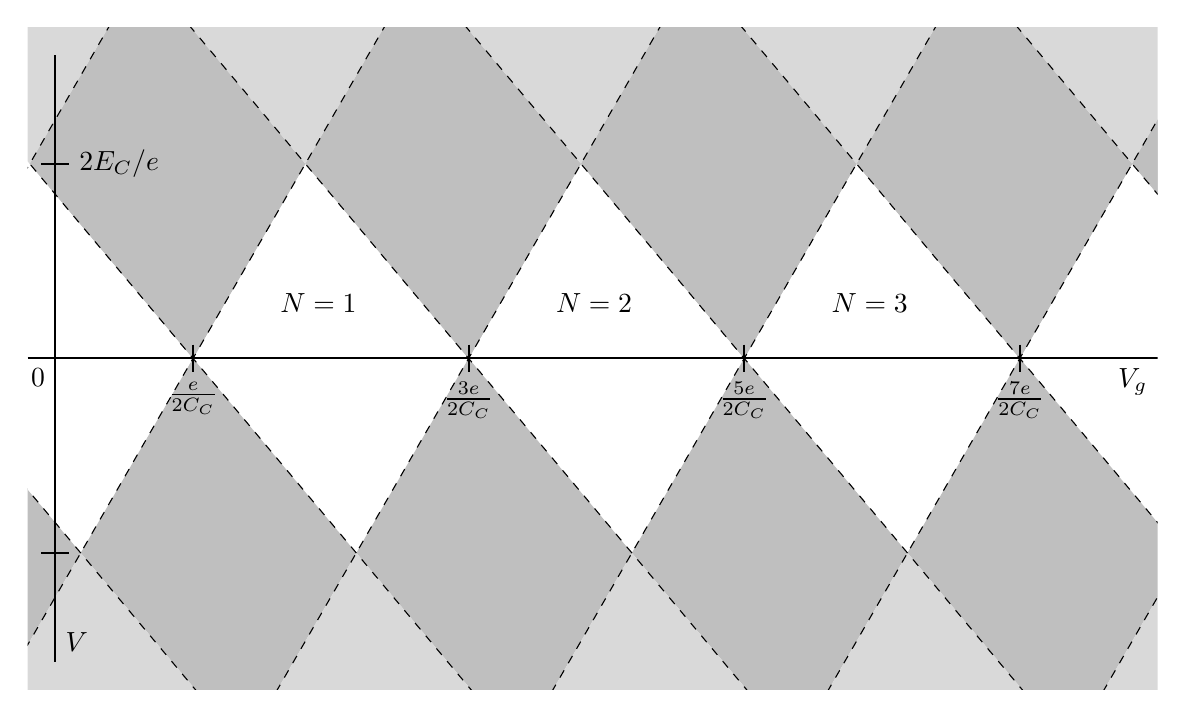
\begin{tikzpicture}[scale=3.5]
    \clip (-0.1,-1.2) rectangle (4,1.2);

    % White diamonds
    \fill[white] (-0.5,0) -- ++(60:0.815) -- ++(-50:0.922) -- ++(60:-0.815) -- ++(-50:-0.922);
    \fill[white]  (0.5,0) -- ++(60:0.815) -- ++(-50:0.922) -- ++(60:-0.815) -- ++(-50:-0.922);
    \fill[white]  (1.5,0) -- ++(60:0.815) -- ++(-50:0.922) -- ++(60:-0.815) -- ++(-50:-0.922);
    \fill[white]  (2.5,0) -- ++(60:0.815) -- ++(-50:0.922) -- ++(60:-0.815) -- ++(-50:-0.922);
    \fill[white]  (3.5,0) -- ++(60:0.815) -- ++(-50:0.922) -- ++(60:-0.815) -- ++(-50:-0.922);

    \fill[lightgray] (-0.5,0) ++(60:-0.815) -- ++(60:0.815) -- ++(-50:0.922) -- ++(60:-0.815) -- ++(-50:-0.922);
    \fill[lightgray]  (0.5,0) ++(60:-0.815) -- ++(60:0.815) -- ++(-50:0.922) -- ++(60:-0.815) -- ++(-50:-0.922);
    \fill[lightgray]  (1.5,0) ++(60:-0.815) -- ++(60:0.815) -- ++(-50:0.922) -- ++(60:-0.815) -- ++(-50:-0.922);
    \fill[lightgray]  (2.5,0) ++(60:-0.815) -- ++(60:0.815) -- ++(-50:0.922) -- ++(60:-0.815) -- ++(-50:-0.922);
    \fill[lightgray]  (3.5,0) ++(60:-0.815) -- ++(60:0.815) -- ++(-50:0.922) -- ++(60:-0.815) -- ++(-50:-0.922);

    \fill[lightgray]  (0.5,0) ++(-50:-0.922) -- ++(60:0.815) -- ++(-50:0.922) -- ++(60:-0.815) -- ++(-50:-0.922);
    \fill[lightgray]  (1.5,0) ++(-50:-0.922) -- ++(60:0.815) -- ++(-50:0.922) -- ++(60:-0.815) -- ++(-50:-0.922);
    \fill[lightgray]  (2.5,0) ++(-50:-0.922) -- ++(60:0.815) -- ++(-50:0.922) -- ++(60:-0.815) -- ++(-50:-0.922);
    \fill[lightgray]  (3.5,0) ++(-50:-0.922) -- ++(60:0.815) -- ++(-50:0.922) -- ++(60:-0.815) -- ++(-50:-0.922);
    \fill[lightgray]  (4.5,0) ++(-50:-0.922) -- ++(60:0.815) -- ++(-50:0.922) -- ++(60:-0.815) -- ++(-50:-0.922);

    \fill[lightgray!60] (-0.5,0) ++(60:-0.815) ++(-50:0.922) -- ++(60:0.815) -- ++(-50:0.922) -- ++(60:-0.815) -- ++(-50:-0.922);
    \fill[lightgray!60]  (0.5,0) ++(60:-0.815) ++(-50:0.922) -- ++(60:0.815) -- ++(-50:0.922) -- ++(60:-0.815) -- ++(-50:-0.922);
    \fill[lightgray!60]  (1.5,0) ++(60:-0.815) ++(-50:0.922) -- ++(60:0.815) -- ++(-50:0.922) -- ++(60:-0.815) -- ++(-50:-0.922);
    \fill[lightgray!60]  (2.5,0) ++(60:-0.815) ++(-50:0.922) -- ++(60:0.815) -- ++(-50:0.922) -- ++(60:-0.815) -- ++(-50:-0.922);
    \fill[lightgray!60]  (3.5,0) ++(60:-0.815) ++(-50:0.922) -- ++(60:0.815) -- ++(-50:0.922) -- ++(60:-0.815) -- ++(-50:-0.922);

    \fill[lightgray]  (0.5,0) ++(-50:-0.922) -- ++(60:0.815) -- ++(-50:0.922) -- ++(60:-0.815) -- ++(-50:-0.922);
    \fill[lightgray]  (1.5,0) ++(-50:-0.922) -- ++(60:0.815) -- ++(-50:0.922) -- ++(60:-0.815) -- ++(-50:-0.922);
    \fill[lightgray]  (2.5,0) ++(-50:-0.922) -- ++(60:0.815) -- ++(-50:0.922) -- ++(60:-0.815) -- ++(-50:-0.922);
    \fill[lightgray]  (3.5,0) ++(-50:-0.922) -- ++(60:0.815) -- ++(-50:0.922) -- ++(60:-0.815) -- ++(-50:-0.922);
    \fill[lightgray]  (4.5,0) ++(-50:-0.922) -- ++(60:0.815) -- ++(-50:0.922) -- ++(60:-0.815) -- ++(-50:-0.922);

    \fill[lightgray!60]  (0.5,0) ++(-50:-0.922) ++(-50:-0.922) -- ++(60:0.815) -- ++(-50:0.922) -- ++(60:-0.815) -- ++(-50:-0.922);
    \fill[lightgray!60]  (1.5,0) ++(-50:-0.922) ++(-50:-0.922) -- ++(60:0.815) -- ++(-50:0.922) -- ++(60:-0.815) -- ++(-50:-0.922);
    \fill[lightgray!60]  (2.5,0) ++(-50:-0.922) ++(-50:-0.922) -- ++(60:0.815) -- ++(-50:0.922) -- ++(60:-0.815) -- ++(-50:-0.922);
    \fill[lightgray!60]  (3.5,0) ++(-50:-0.922) ++(-50:-0.922) -- ++(60:0.815) -- ++(-50:0.922) -- ++(60:-0.815) -- ++(-50:-0.922);
    \fill[lightgray!60]  (4.5,0) ++(-50:-0.922) ++(-50:-0.922) -- ++(60:0.815) -- ++(-50:0.922) -- ++(60:-0.815) -- ++(-50:-0.922);

    % Axis
    \draw[thick] (0,-1.1) node[above right]{\(V\)} -- (0,1.1);
    \draw[thick] (-0.05, 0.706) -- ++(0.1,0) node[right]{\(2E_{C}/e\)};
    \draw[thick] (-0.05, -0.706) -- ++(0.1,0);% node[right]{\(-2E_{C}\)};

    \draw[thick] (-0.1,0) -- (4,0) node[below left]{\(V_{g}\)};
    \draw[thick] (0.5, 0.05) -- ++(0,-0.1) node[below]{\(\frac{e}{2C_{C}}\)};
    \draw[thick] (1.5, 0.05) -- ++(0,-0.1) node[below]{\(\frac{3e}{2C_{C}}\)};
    \draw[thick] (2.5, 0.05) -- ++(0,-0.1) node[below]{\(\frac{5e}{2C_{C}}\)};
    \draw[thick] (3.5, 0.05) -- ++(0,-0.1) node[below]{\(\frac{7e}{2C_{C}}\)};
    \draw[thick] (0,0) node[below left]{\(0\)};

    \draw[thick] (0.955,0.2) node[]{\(N = 1\)};
    \draw[thick] (1.955,0.2) node[]{\(N = 2\)};
    \draw[thick] (2.955,0.2) node[]{\(N = 3\)};

    % Diamond edges
    \draw[dashed] (-0.5,0) ++( 60:-2) -- ++( 60:4);
    \draw[dashed] (0.5,0)  ++( 60:-2) -- ++( 60:4);
    \draw[dashed] (1.5,0)  ++( 60:-2) -- ++( 60:4);
    \draw[dashed] (2.5,0)  ++( 60:-2) -- ++( 60:4);
    \draw[dashed] (3.5,0)  ++( 60:-2) -- ++( 60:4);
    \draw[dashed] (4.5,0)  ++( 60:-2) -- ++( 60:4);
    \draw[dashed] (-0.5,0) ++(-50:-2) -- ++(-50:4);
    \draw[dashed] (0.5,0)  ++(-50:-2) -- ++(-50:4);
    \draw[dashed] (1.5,0)  ++(-50:-2) -- ++(-50:4);
    \draw[dashed] (2.5,0)  ++(-50:-2) -- ++(-50:4);
    \draw[dashed] (3.5,0)  ++(-50:-2) -- ++(-50:4);
    \draw[dashed] (4.5,0)  ++(-50:-2) -- ++(-50:4);
\end{tikzpicture}
\caption{Coulomb diamonds in an SET due to Coulomb blockade. As we move
towards the left, more charges are stored into the conducting island.}
\label{fig:CoulombDiamonds}
\end{figure}

For a process to occur, the variation in energy of that process needs to be
less than \(0\). Since we are interested in the transportation of charge
through the SET, we want electrons flowing through one side to the other,
which means \(\Delta E_{IL}, \Delta E_{OR} < 0\) or
\(\Delta E_{IR}, \Delta E_{OL} < 0\). In figure \ref{fig:CoulombDiamonds}
we can see a plot of this in the \(V-V_{g}\) plane, with the white
diamonds being where no condition is met, and darker diamonds
being we are specifically \(\Delta E_{IL}(N), \Delta E_{OR}(N+1) < 0\) and
\(\Delta E_{IR}(N), \Delta E_{OL}(N+1) < 0\).

With this we have enough information to have a basic understanding of how a
SET works:
\begin{itemize}
    \item For the SET to operate as it should, \(|V|\) needs to be lower than
        \(2E_{C}/e\). If not, the current can not be turned off, and we cannot
        ensure that it is a one electron current. Picturing this scenario
        with the energy levels inside the conducting island it makes perfect
        sense. If \(|V| > 2E_{C}/e\), the energy drop from one terminal to the
        other will be greater than the spacing between levels, ensuring
        that there is always an empty level to fill or a full level to empty.
    \item Using the same logic as the previous point, the thermal energy of
        the leads and the island must be smaller than \(E_{C}\), since
        the thermal energy raises the available energy to mobilize while
        not increasing the required energy to move, giving effectively
        extra voltage to the system.
    \item The activation window for \(V_{g}\) is inversely proportional to
        \(V\), and it occurs when thanks to \(V_{g}\), an energy level
        is placed between \(0\) and \(V\).
\end{itemize}

If we want to use a SET for spin sensing in a quantum dot, first we need to
use it for charge sensing. This is done by connecting via a capacitor the
conducting island of the SET with the QD. When a charge is placed in the QD, it
will influence the SET by, effectively, adding a bias to \(V_{g}\). Choosing
\(V\) and \(V_{g}\) appropriately for the bias that the charge introduces, we
can tune the SET to make it let the current flow when a charge is present
and stop it when it is absent (or the opposite).

For spin sensing, what we do is set up our system in such a way that the charge
in the QD and the spin of that charge are correlated. This process is called
spin to charge conversion, and there are mainly 2 ways of doing it:

\begin{itemize}
    \item \textbf{Elzerman readout:} After inducing a Zeeman splitting in the
        QD, we can connect to it with a tunnel junction a reservoir,
         with a Fermi energy in between both spin states in the
        QD. If we detect a fluctuation in charge, it means the electron
        decayed through the reservoir to the lowest energy spin state. If
        not, it means it already was in the lowest energy spin state.
    \item \textbf{Pauli Spin Blockade:} By connecting to our QD another QD via a tunnel junction
        with lower energy and an electron with known spin, we can infer the
        spin in the first QD based on if a tunneling event occurred, thanks
        to the Pauli exclusion principle.
\end{itemize}

To summarize, a SET is a transistor that thanks to Coulomb blockade,
a discretization on the energy spectrum of conducting islands due to
Coulomb repulsion, is able to let a single electron current through and
control it. It is main operation conditions are \(e^2/C_{\Sigma} \gg V\)
and \(e^2/2C_{\Sigma} \gg k_{b}T\), with \(V\) the voltage applied,
\(C_{\Sigma}\) the capacitance of the conducting island of the SET, \(k_{b}\)
the Boltzmann constant and \(T\) the temperature of the SET, and when current
flows, its resistance must be such that \(R \gg 51.6\unit{\kilo\ohm}\).

By connecting a quantum dot to we can measure the charge inside it, and
by implementing a spin to charge conversion scheme we can also measure
the spin of said charge.

\newpage
\subsection{RF reflectometry}
\label{subsec:RFRef}
Radio frequency reflectometry is a method to measure change in an impedance
connected to a transmission line via the reflection of a radio signal.

Usual lumped element treatment of AC circuits assumes that the size of the
circuit is small with respect to the wavelength of the voltage,
but with radio frequency voltages we cannot do that. The main consequences for
us are:
\begin{itemize}
    \item Now voltage and current are dependent on how far along the circuit
    you are, due to how fast it changes with respect to the size of the circuit
    itself (\(V(t), I(t) \rightarrow V(x, t), I(x, t)\))
\item The intrinsic inductance and capacitance per unit length of a long
    connection cannot be ignored
\end{itemize}

In such cases those connections are made with what is known as a
transmission line, which is a cable designed to minimize the radiation of
power via that inductance and capacitance, and includes a signal and a
ground connection in one package. One example of a transmission line would be a
coaxial cable, in which the central conductor is the signal and the outer jacket
ground.

\begin{figure}[t]
\centering
\begin{circuitikz}[]
    \newcommand{\lenghOfTransmissionLine}{6}
    \draw (0,0) node[ground]{};
    \draw (0,0) to[sV] ++(0,1.5) to[short] ++(1.5,0);
    \draw (1.5,0) to[capacitor] ++(0,1.5) to[L] ++(1.5,0) to[short] ++(0.5,0);
    \foreach \i in {2,...,\lenghOfTransmissionLine}{
        \draw (2*\i - 0.5,0) to[capacitor] ++(0,1.5) to[L] ++(1.5,0) to[short] ++(0.5,0);
    }
    \draw ({2*(1+\lenghOfTransmissionLine)-0.5},0) node[ground]{};
    \draw ({2*(1+\lenghOfTransmissionLine)-0.5},1.5) to[generic, l=\(Z\)] ++(0,-1.5);
    \draw (0,0) to[short] ++({2*(1+\lenghOfTransmissionLine)-0.5},0);
    \draw[dashed] (0.93,-0.15) rectangle ++(2,2);
    \draw [latexslim-latexslim] (2.93,-0.35) -- node[below] {\(\Delta x\)} ++(-2,0);
\end{circuitikz}
\caption{Lumped element model of a lossless transmission line connected to a
    generic impedance \(Z\). In order to model the relevant
    impedance per unit length of the transmission line at radio frequencies,
    we represent it via sections with inductors in series and capacitors
    in parallel. Each periodic section like the one inside the dashed rectangle
    represents a segment of length \(\Delta x\) of the transmission line.}
\label{fig:LumpedTransmisionLine}
\end{figure}

Even though a transmission line minimizes that radiation of power, it does not
erase it, and we need to take it into account in our calculations. To model this
inductance and capacitance per unit length (\(L_{l}\) and \(C_{l}\) respectively),
we will discretize it via a lumped element representation like in figure
\ref{fig:LumpedTransmisionLine}, ignoring the losses by not including any
resistance  in our circuit.
Each pair inductor-capacitor will occur along a length \(\Delta x\) of the
transmission line, so their inductance and capacitance in that stretch will be
\(L = \Delta x \cdot L_{l}\) and \(C = \Delta x \cdot C_{l}\). Applying Kirchhoff
at a point \(x\) in the transmission line we get
\begin{align*}
    V(x+\Delta x, t) - V(x, t) &= -\Delta x L_{l} \frac{\partial I}{\partial t}\\
    I(x+\Delta x, t) - I(x, t) &= -\Delta x C_{l} \frac{\partial V}{\partial t}\\
\end{align*}
And doing the limit \(\Delta x \to 0\) gives us the telegraph equations for a
lossless transmission line
\begin{align}
\begin{split}
\label{eq:TelegraphEq}
    \frac{\partial V}{\partial x} = - L_{l}\frac{\partial I}{\partial t}\\
    \frac{\partial I}{\partial x} = - C_{l}\frac{\partial V}{\partial t}\\
\end{split}
\end{align}
With solutions
\begin{align*}
\begin{split}
    \label{eq:TelegraphSol}
    V(x,t) &= V_{+}(t - x/v_{p}) + V_{-}(t + x/v_{p})))\\
    I(x,t) &= \frac{1}{Z_{0}}(V_{+}(t - x/v_{p}) - V_{-}(t + x/v_{p}))
\end{split}
\end{align*}

Where \(v_{p} = \frac{1}{\sqrt{L_{l}C_{l}}}\) is the phase velocity of the wave,
\(Z_{0} = \sqrt{\frac{L_{l}}{C_{l}}}\) is the characteristic impedance of the
line and \(V_{+}\) and \(V_{-}\) are generic functions that describe a right
and left traveling wave respectively. Since we will be choosing our reference
frame such that our signal will be always traveling from left to right, the
appearance of \(V_{-}\) in our calculations will mean a reflection.

If we add a generic impedance \(Z\) at the end of the transmission line, we
add the boundary condition
\begin{equation*}
\label{eq:RfBoundCond}
    \frac{V(x_{\text{End}},\omega)}{I(x_{\text{End}},\omega)} = Z(\omega)
\end{equation*}
With \(V(x,\omega)\) and \(I(x,\omega)\) being the time Fourier transforms of
\(V(x,t)\) and \(I(x,t)\) respectively. Choosing \(x=x_{\text{End}}=0\) to
simplify and using the time Fourier transforms of expressions
\ref{eq:TelegraphEq}, we get
\begin{equation}
\label{eq:TelegraphEqFourierWithBound}
    \frac{V(0,\omega)}{I(0,\omega)} =
    Z_{0}\frac{V_{+}(\omega) + V_{-}(\omega)}
    {V_{+}(\omega) - V_{-}(\omega)} = Z(\omega)
\end{equation}

As we can see, the only way in which \(Z_{0} = Z(\omega)\) is if
\(V_{+,-}(\omega)=0\), or in other words, the only way to not get a reflection
is to match \(Z_{0}\) to \(Z(\omega)\). A useful parameter to define is the
reflection coefficient \(\Gamma = \frac{V_{-}(\omega)}{V_{+}(\omega)}\), and
with equality \ref{eq:TelegraphEqFourierWithBound} has the form
\begin{equation}
\label{eq:ReflecCoeff}
    \Gamma = \frac{Z(\omega) - Z_{0}}{Z(\omega) + Z_{0}}
\end{equation}

This reflection coefficient is the key to RF reflectometry, because if we
know the characteristic impedance of our transmission line, we can measure
the power and the phase reflected and obtain \(Z(\omega)\).

If we want to measure 2 distinct impedances, and we want to maximize the
reliability of our measure, the obvious way to do it would be to make the values
of \(\Gamma\) be as separated as possible. A more formal way to express this
idea is through the signal-to-noise ratio (SNR)\cite{vigneauProbingQuantumDevices2023} of the measurement

\begin{equation}
\label{eq:SNR}
\text{SNR} = |\Delta\Gamma|^2\frac{P_{0}}{P_{N}}
\end{equation}

With \(P_{0}\) and \(P_{N}\) the power of the signal and noise respectively and
\(\Delta\Gamma = \Gamma_{B} - \Gamma_{A}\) the difference in reflection
coefficients between the two states to measure, whose modulus is what is
called the contrast. If we want to improve our measurements, we need to
increase our SNR.

\newpage
\subsection{Kinetic inductance and his nonlinearity}
\label{subsec:KineticInductance}
Due to the high mobility of the charge carriers in a super conductor, a phenomenon
known as kinetic inductance emerges. This name comes from the fact that as opposed
to a usual inductor, which functions by storing energy in the magnetic field
generated by the charge carriers, it is stored as the kinetic energy of the
charge carriers themselves.

With this simple definition of the kinetic inductance and a little bit of
Drude and Ginzburg-Landau theory, we have all we need to derive the property
that interests us the most: it's nonlinearity.

The energy stored by an inductor of inductance \(L\) is

\begin{equation*}
\label{eq:InductiveEnergy}
    E = \frac{1}{2}LI^2
\end{equation*}

So, in the case of the kinetic inductance of length \(l\) and cross-section \(S\)

\begin{equation*}
\label{eq:KineticInductiveEnergy}
    E_{k} = \frac{1}{2}L_{k}I^2 = \frac{1}{2}m(nlS)v^2
\end{equation*}

With \(n\), \(m\) and \(v\) the volumetric density, the mass and the speed of
the charge carriers. By solving for \(L_{k}\) and defining the
current density as \(j=nqv\) with \(q\) the charge of the charge carriers
we arrive at the following expression

\begin{equation*}
\label{eq:LkOfn}
    L_{k} = \frac{mlj^2}{nq^2Sj^2} = \frac{ml}{q^2S}\frac{1}{n}
\end{equation*}

Now, using the Ginzburg-Landau expression for the volumetric density of supercharge
carriers

\begin{equation*}
\label{eq:GLn}
    n(v) = |\Psi|^2 = \frac{1}{\beta}\left[|\alpha| - \frac{1}{2}m v^2\right]
\end{equation*}

And doing a second order approximation of \(L_{k}\) at \(v \approx 0\), we arrive
at our desired expression

\begin{equation}
\label{eq:KineticNonLineality}
    L_{k} = L_{k0}\left(1 + \frac{j^2}{j_{*}^2} + \dots\right)
\end{equation}

With \(L_{k0} = \frac{ml}{q^2Sn(v=0)}\) and \(j_{*}^2 =
\frac{2q^2|\alpha|^3}{m\beta^2}\). If we compare \(j_{*}\)
to the critical current \(j_{c}\), which is the maximum current that
the system can withstand and can be calculated by obtaining the maximum of
\(j\) with respect to \(v\), we get that

\begin{equation*}
    j_{*} = \sqrt{\frac{27}{4}}j_{c}
\end{equation*}

With this we can not only see that the kinetic inductance has a quadratic
dependence with the current, but that the sensibility of that dependence it is
given by the critical current of the material.

But, the applications of inductors are usually with AC voltages, and in that
case our kinetic inductance would be varying constantly. How can we use the
kinetic inductor then?

The solution is to introduce a DC bias to the circuit, with an intensity much
greater than the maximum of the AC current, but still small enough to not break
superconductivity and to use an AC current much smaller than the critical current.
With it, we can have an inductor that changes inductance along with the resistance
of the SET, since the effects of the AC current can be ignored.

\begin{align*}
\begin{split}
L_{k} &= L_{k0}\left(1 + \frac{(j_{AC} + j_{DC})^2}{j_{*}^2} + \dots\right)\\
      &= L_{k0}\left(1 + \frac{j_{DC}^2}{j_{*}^2} + \frac{j_{DC}j_{AC}}{j_{*}^2} + 
      \frac{j_{AC}^2}{j_{*}^2} + \dots\right)\\
      &= L_{k0}\left(1 + \frac{j_{DC}^2}{j_{*}^2} + (\frac{j_{DC}}{j_{*}} + 
      \frac{j_{AC}}{j_{*}})\frac{j_{AC}}{j_{*}} + \dots\right)\\
      &= L_{k0}\left(1 + \frac{j_{DC}^2}{j_{*}^2} + \dots\right)
      \text{ since \(j_{DC} < j_{c}\) and \(j_{AC} \ll j_{c}\)}
\end{split}
\end{align*}


\end{document}
